\part{Asynchronous RL}
For agentic workloads, especially long-horizon tasks, rollout lengths are highly variable, so short trajectories finish quickly while long ones become stragglers.

Asynchronous RL algorithms are proposed to mitigate this imbalanced generation overhead by consuming rollouts continuously as they arrive, improving utilization and wall-clock efficiency. However, asynchrony introduces one challenge, where each trajectory can be generated by multiple versions of the old rollout model, which leads to more unpredictable and severe off-policy, and thus harms the training stability.

Recall that in the Standard PPO, the objective is defined as
\begin{align*}
     \max_{\theta} \Jcal_{\text{PPO-clip}}(\theta):= \Embb_{\tau\sim \pi_{\theta_{\text{old}}}}\left[ \sum_{t=0}^{T-1}  \min\left\{\frac{\pi_{\theta}(a_t|s_t)}{\pi_{\theta_{\text{old}}}(a_t|s_t)}\hat A_\phi(s_t,a_t), \operatorname{clip}\left(\frac{\pi_{\theta}(a_t|s_t)}{\pi_{\theta_{\text{old}}}(a_t|s_t)}, 1-\epsilon, 1+\epsilon\right)\hat A_\phi(s_t,a_t)\right\}\right],
\end{align*}

controls policy update size via the ratio $\frac{\pi_{\theta}}{\pi_{\theta_{\text{old}}}}$, where $\pi_{\theta_{\text{old}}}$ is assumed to be both the \textit{proximal policy} (the anchor policy for PPO clipping) and the \textit{behavior policy} (the policy that collected the data); both terms are defined in \citep{hilton2022batchsizeinvariancepolicyoptimization}, which was primarily proposed to achieve batch size-invariance for PPO.

The key idea is to decouple these two roles. Let $\pi_{\theta_{\text{prox}}}$ denote the proximal policy that anchors the clipping region, and let $\pi_{\theta_{\text{beh}}}$ denote the behavior policy that collected the trajectories. Then a three-policy version of PPO-Clip can be written as
\begin{align*}
    \max_{\theta}\Jcal_{\text{PPO-Decoupled}}(\theta)
    :=
    \Embb_{\tau\sim \pi_{\theta_{\text{beh}}}}
    \left[
        \sum_{t=0}^{T-1}
        w_t
        \min\left\{
            r_t(\theta)\hat A_\phi(s_t,a_t),
            \operatorname{clip}\left(r_t(\theta),1-\epsilon,1+\epsilon\right)\hat A_\phi(s_t,a_t)
        \right\}
    \right],
\end{align*}
where
\begin{align*}
    w_t
    :=
    \frac{\pi_{\theta_{\text{prox}}}(a_t|s_t)}
    {\pi_{\theta_{\text{beh}}}(a_t|s_t)},
    \qquad
    r_t(\theta)
    :=
    \frac{\pi_{\theta}(a_t|s_t)}
    {\pi_{\theta_{\text{prox}}}(a_t|s_t)}.
\end{align*}
Here, $w_t$ is the importance sampling correction from the behavior policy to the proximal policy. During one policy update, $\pi_{\theta_{\text{prox}}}$ and $\pi_{\theta_{\text{beh}}}$ are fixed, so $w_t$ is treated as a constant with respect to $\theta$. In contrast, $r_t(\theta)$ is the PPO ratio used to control how far the current policy $\pi_\theta$ moves away from the proximal policy $\pi_{\theta_{\text{prox}}}$.

\textbf{Remark}
\begin{itemize}
    \item If $\pi_{\theta_{\text{beh}}}=\pi_{\theta_{\text{prox}}}=\pi_{\theta_{\text{old}}}$, then $w_t=1$ and the objective reduces to the standard PPO-Clip objective.
    \item The behavior policy $\pi_{\theta_{\text{beh}}}$ can be stale or generated by a different worker, while the update size is still controlled relative to $\pi_{\theta_{\text{prox}}}$
    \item The clipping mechanism is preserved because the clipped ratio is $r_t(\theta)=\pi_{\theta}(a_t|s_t)/\pi_{\theta_{\text{prox}}}(a_t|s_t)$, not the behavior correction $w_t$.
\end{itemize}

For the asynchronous discussion, it is clearer to write the proximal policy as $\pi_{\theta_{\text{old}}}$ and the behavior policy as $\pi_{\theta_{\text{rollout}}}$. The policy $\pi_{\theta_{\text{old}}}$ is the frozen PPO anchor used in the clipping ratio, while $\pi_{\theta_{\text{rollout}}}$ is the model that actually generated the sampled token or action. For more details, see the \href{https://verl.readthedocs.io/en/latest/algo/rollout_corr_math.html#implementation-in-verl-the-three-policy-framework}{veRL} discussion and the \href{https://github.com/THUDM/slime}{Slime} reference implementation.


Consequently, the data consumed by a trainer update may not have a single behavior policy. Some trajectories may have been generated before the rollout engine refreshed, while later trajectories may use the refreshed rollout weights; in a long rollout, even different tokens in the same trajectory can correspond to different rollout snapshots. See \autoref{fig:async.rollout.policy.lag} for a visualization. 
\begin{figure}[H]
    \centering
    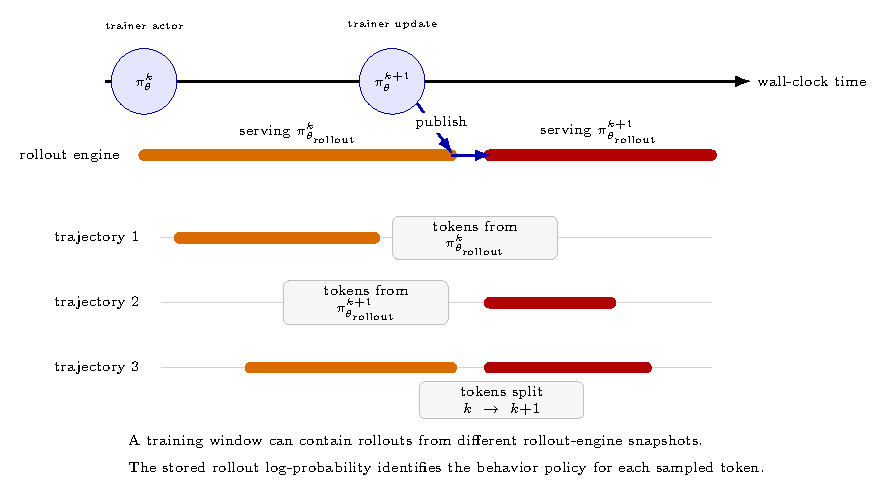
\includegraphics[width=0.9\linewidth]{figures/async_rollout_policy_lag.pdf}
    \caption{Policy lag comes from the time gap between the trainer actor update and the rollout engine refresh. During this gap, the trainer has advanced to $\pi_\theta^{k+1}$ while the rollout engine may still generate tokens with $\pi_{\theta_{\mathrm{rollout}}}^{k}$; after refresh, later tokens are generated with $\pi_{\theta_{\mathrm{rollout}}}^{k+1}$. A trajectory that spans the refresh can therefore contain tokens from both rollout snapshots.}
    \label{fig:async.rollout.policy.lag}
\end{figure}

Thus, exact off-policy correction requires the behavior probability for the particular sampled token/action, namely the rollout-time value $\pi_{\theta_{\text{rollout}}}(a_t|s_t)$ used when that token/action was sampled. In practice, this means storing the rollout log-probability together with each generated token. If these log-probabilities are not stored, then one would need to keep enough rollout-policy checkpoints to recompute them later. The required history is therefore a history of behavior probabilities, or equivalently rollout-policy snapshots. In the long horizon setting, maintaining the history is not feasible in practice.

In this part, we discuss various asynchronous RL algorithms target to address various issues arised in the asynchronous RL.